\documentclass[12pt,BSc,wordcount,twoside]{muthesis}
% The regulations say that 12pt should be used
% Change the MSc option to MPhil, MRes or PhD if appropriate
% Add 'anon' to the above options to replace your name with your student ID
\usepackage{verbatim}
\usepackage{graphicx}
\usepackage{url} % typeset URL's reasonably
\usepackage{listings}

\usepackage{pslatex} % Use Postscript fonts

% Uncomment the next line if you want subsubsections to be numbered
\setcounter{secnumdepth}{3}
% Uncomment the next line if you want subsubsections to be appear in
% the table of contents
\setcounter{tocdepth}{3}

% Uncomment the following lines if you want to include the date as a
% header in draft versions
%\usepackage{fancyhdr}
%\pagestyle{fancy}
%\lhead{}  % left head
%\chead{Draft: \today} % centre head
%\lfoot{}
%\cfoot{\thepage}
%\rfoot{}

\begin{document}
% Uncomment the following lines to leave out list of figures, tables
% and copyright until final printing
%\figurespagefalse
%\tablespagefalse
%\copyrightfalse

\title{Mitigating IPC Overhead in the seL4 Microkernel:\\
Design, Implementation, and Evaluation of an Asynchronous, Multiclient File Server}
\author{Luke Rule}
\stuid{11012731}
\principaladviser{James Garside}

\beforeabstract

\prefacesection{Abstract}
This dissertation presents the design, implementation and evaluation of a multiclient file server upon the seL4 Microkit framework, motivated by the aim of mitigating IPC overhead, a key performance constraint in microkernel-based systems, through asynchronous client-server communication. The system supports a rich set of FS operations, including namespace, data and metadata management, and multiclient access control.

The file server is structured around modular and flexible core abstractions including blocks, inodes, directories and file descriptors, providing clear separation between persistent FS metadata and per-client runtime state. Two communication models are implemented over this core system: a synchronous model based on protected procedure calls, and an asynchronous model based on notifications, shared memory queues and batched request processing. A transparent API abstracts communication details while preserving consistent operation semantics across both models.

The asynchronous model demonstrated reduced IPC overhead through batching and reduced synchronisation frequency, improving throughput and lowering average operation latency under suitable workloads. However, these benefits are workload-dependent, with limited gains under highly interdependent workloads. A key insight is that communication structure alone can significantly influence system behaviour independently of core FS design. The results further suggest that, although evaluated in a single-threaded environment, the asynchronous design could enable substantially greater concurrent processing on multicore systems through non-blocking execution and overlap of request generation, servicing and response handling.

The work demonstrates that complex, stateful services can be realised entirely in user space within the Microkit framework for seL4, and provides insight into trade-offs between synchronous and asynchronous communication for future microkernel-based system services.




\afterabstract

\prefacesection{Acknowledgements}
I would like to thank...

\prefacesection{Abbreviations}
\begin{tabular}{ll}
  ABI   & Application Binary Interface \\
  API   & Application Programming Interface \\
  CPU   & Central Processing Unit \\
  DMA   & Direct Memory Access \\
  IPC   & Inter-Process Communication \\
  IRQ   & Interrupt Request \\
  MMIO  & Memory-Mapped Input/Output \\
  OS    & Operating System \\
  POSIX & Portable Operating System Interface \\
  RAM   & Random Access Memory \\
  RPC   & Remote Procedure Call \\
  TCB   & Thread Control Block \\
  VFS   & Virtual File System \\
\end{tabular}


\afterpreface

% These include the actual text
\chapter{Introduction}
\label{cha:intro}


\section{Context and Motivation}
Modern software systems are larger, more complex, and more interdependent than ever before[], placing significant demands upon the operating systems that underpin them. Contemporary mainstream operating systems, such as Windows, Linux, and macOS, are largely based upon monolithic kernel designs[], where the majority of system functionality resides in a single privileged address space. This key characteristic enables high performance[], yet it comes at the cost of scalability, security and robustness[], as it requires forming a large trusted computing base (TCB) where a single fault can compromise the entire system[].
\newline \newline Simultaneously, modern software and hardware architectures are increasingly employing modularity, isolation, and concurrency[]. Distributed systems, cloud-native microservices, and data centre-scale applications all decompose functionality into loosely-coupled components[], and most current hardware performance scaling is driven by multi-core and many-core parallelism[]. These trends place pressure on operating system design to provide stronger security guarantees and better support for concurrent, component-based execution.
\newline \newline Microkernel design naturally aligns with these requirements[]. By minimising kernel functionality and moving most non-essential services, such as device drivers and file systems, into user space, microkernels reduce the TCB significantly and enforce separation between components. Yet, this modularity requires costly inter-process communication (IPC), which incurs overhead from context switching, data transfer, and cache disruption[]. 
\newpage \noindent The L4 family of microkernels addressed this bottleneck by substantially reducing IPC costs through aggressive kernel minimisation and IPC fastpath design[]; yet, despite these advances, IPC overhead remains a fundamental constraint in microkernel-based systems and a barrier to their wider adoption[]. By combining these performance improvements with strong security guarantees through formal verification[], however, the seL4 microkernel represents a significant step toward making microkernel-based designs viable for real-world deployment, particularly in security and safety-critical domains[]. Still, performance constraints remain a limiting factor, especially for high-frequency IPC workloads.
\newline \newline One of the most frequently accessed operating system services is the file server[], which acts as the primary interface for persistent storage and data exchange. File system operations are both latency-sensitive and IPC-intensive[], making them critical to overall system performance in microkernel environments. In synchronous architectures, even simple file operations may involve multiple IPC invocations between the client and the file server, amplifying the impact of communication overhead.
\newline \newline This report presents the design and implementation of an asynchronous, multiclient file server for the seL4 microkernel, validates its correctness and usability, and evaluates its effectiveness in mitigating IPC overhead. The proposed architecture decouples request submission from response handling, enabling batching of operations, reducing blocking behaviour, and increasing concurrency. These properties have the potential to improve throughput and resource utilisation under both single and multi-client workloads. In addition, beyond serving as an evaluation platform, the implementation constitutes a practical, reusable system component, demonstrating how critical services can be structured within a microkernel environment using the seL4 Microkit’s component-based design model. 


\section{Aims and Objectives}
Building upon the L4 family’s reduction of IPC overhead, and motivated by the increasing importance of concurrency in contemporary systems, this work aims to further mitigate IPC costs by reducing the number of IPC interactions required between components. In doing so, it also seeks to demonstrate the capabilities of the seL4 Microkit framework through the design and implementation of a flexible, user-space file server.
\newpage \noindent This report has the following objectives:
\begin{itemize}
    \item Design and implement a viable file system core capable of supporting a wide range of file and directory operations.
    \item Design and implement an efficient storage model based on inode and block abstractions, supporting effective space utilisation and flexible file and directory representation.
    \item Design and implement a scalable, asynchronous interface enabling concurrent request submissions and completion handling from multiple clients, alongside a synchronous interface to facilitate comparison between communication models.
    \item Design and implement a lightweight client-side library providing a simple and usable abstraction over the file server interface.
    \item Validate the correctness of the file server through comprehensive multi-level testing.
    \item Design and implement a benchmarking framework to evaluate asynchronous file server performance against a synchronous baseline under realistic workloads.
    \item Evaluate the effectiveness of the asynchronous file server architecture in reducing IPC overhead and improving performance, in terms of latency, throughput, and scalability.
\end{itemize}

\section{Evaluation Strategy}
To evaluate the proposed implementation, this work considers both the correctness of file system operations and the performance characteristics of asynchronous queue-based submission compared to synchronous, blocking calls.
\newline \newline Correctness is validated at multiple stages of granularity - unit, integration and end-to-end testing - to ensure file operations correctly persist and return data across a range of scenarios, including edge and error cases.
\newline \newline For performance evaluation, a set of benchmarks are designed to compare the synchronous and asynchronous interfaces under varying workloads and measure key metrics, including latency, throughput, and IPC frequency. Experiments are conducted across different levels of request batching to assess the trade-off between asynchronous overhead in low-batching scenarios and performance gains achieved through reduced IPC at higher batching levels.
\newline \newline The benchmark workloads are designed to approximate realistic file system usage patterns; however, as the system is novel, custom benchmarks are required. While these may not capture all characteristics of production environments, they are sufficient to provide indicative and comparative insights into the performance impact of asynchronous design.


\section{Key Findings}
The evaluation demonstrates that asynchronous communication introduces negligible overhead compared to synchronous execution when no batching is applied, with per-operation latencies remaining effectively equivalent. Crucially, as batching is introduced, significant performance improvements are observed. For single-client workloads, increasing batch sizes reduces per-operation latency by up to ~60\% for reads and ~50\% for writes, demonstrating that reducing IPC frequency has a substantial impact on performance.
\newline \newline These improvements extend to more realistic workloads. In a multi-client benchmark simulating typical file system operations with batching opportunities, the asynchronous model achieves an average latency reduction of approximately 35–40\% compared to the synchronous baseline. Notably, these experiments were conducted on a single core, as current seL4 deployments do not fully utilise multicore execution; consequently, greater throughput would be expected from asynchronous designs in a multicore setting due to increased concurrency, allowing requests to be issued and responses processed in parallel.
\newline \newline However, all evaluations were performed using an in-memory storage model rather than disk-backed persistence. While this isolates IPC and scheduling overhead, real-world performance gains would be less pronounced when incorporating variable disk I/O latency. Nevertheless, the results demonstrate that batching and non-blocking execution can significantly reduce IPC overhead, particularly in high-frequency workloads.

\newpage
\section{Dissertation Structure}
The report begins by presenting the background knowledge required to understand the design of the file server and its architectural context. It then introduces the system design, including the overall architecture, interface models, and key design decisions.
\newline \newline Following this, the implementation of the file server and its two interfaces are described, before outlining the validation strategy and performance evaluation methodology, assessing correctness and comparing the performance of the asynchronous and synchronous communication models.
\newline \newline The report then discusses related work, situating the contribution within existing research, and concludes with a summary of findings, limitations, and directions for future work.





\chapter{Background}
\label{cha:background}

\section{Microkernels}

\subsection{Definition and Characteristics}
Hello, hello hello hello hello hello hello hello hello hello hello hello hello hello hello hello hello hello hello
\subsection{Advantages and Disadvantages}
\subsection{IPC overhead in Microkernels}

\section{seL4 Microkernel}

\subsection{Overview and Design Principles}
\subsection{Architecture and Components}
\subsection{IPC Mechanisms}
\subsection{Use Cases and Applications}
\subsection{Microkit Framework for seL4}


\section{Client-Server Communication}
\subsection{Synchronous Model}
\subsection{Asynchronous Model}

\section{File Servers in Operating Systems}
\subsection{Role and Functionality}
\subsection{Abstractions}
\subsection{Storage and Organisation}
\subsubsection{File Layout}
\subsubsection{Allocation Strategies}
\subsubsection{Metadata Organisation}
\subsection{Client Management}

\section{Related Work}
\subsection{IPC Optimisation Techniques in Microkernels}
\subsection{Asynchronous vs Synchronous Server Designs}
\subsection{File Servers in Microkernel-based Systems}
\subsection{Identified Gaps}

\chapter{Design}
\label{cha:design}

This section describes the design of the file server, including both the interface through which clients interact with the system and the internal file system structure. As both components significantly influence how operations are issued and processed, their design plays a key role in overall system behaviour. 

\section{System Requirements and Constraints}

The design of the file server is driven by both functional requirements and the constraints imposed by Microkit and seL4. These requirements define the intended behaviour of the system, while the constraints shape the design decisions necessary to achieve this within the given environment.

From a functional perspective, the system is required to provide a core set of file system operations, including creation, reading, writing and deletion of files, alongside support for directory structures and getting and setting of associated metadata such as permissions and file size. The system must present a consistent and simple interface to clients, ensuring that operations are executed correctly and that appropriate error codes are returned in response to invalid inputs or failure conditions.

A key requirement of the system is support for multiple clients operating concurrently. The file server must therefore be capable of handling requests from multiple independent clients, maintaining correctness and consistency in the presence of interleaved operations. In addition, the system must support both synchronous and asynchronous interaction models. This will enable direct comparison between traditional blocking request–response behaviour and the proposed asynchronous, batched approach.

Performance is a central non-functional requirement. In particular, the system is designed to minimise the overhead associated with IPC, which is a known bottleneck in microkernel-based systems\cite{}. The asynchronous design must therefore enable efficient batching of operations, reducing the number of required IPC interactions and improving overall throughput. 

Several constraints significantly influence the system design. The Microkit framework enforces a statically defined system configuration to aid high-assurance and high-performance system development, meaning that all protection domains, communication channels and memory regions must be specified at build time. As a result, the number of clients and their associated resources are fixed, hindering the system's ability to adapt.

The IPC model provided by seL4 is inherently synchronous, with communication occurring through blocking interactions. This motivates the use of shared memory and notification mechanisms to enable non-blocking request submission and completion handling.

Hence, memory cannot be shared dynamically between protection domains, preventing the use of copy-free mechanisms that rely on on-demand sharing. Consequently, all data transfer must occur through these shared memory regions, requiring explicit buffer management within the interface design.

Further constraints arise from the execution environment. For development simplicity, the system operates with no access to persistent storage, resulting in a purely in-memory file system. Additionally, due to seL4 constraints, execution is limited to a single core, restricting the ability to exploit parallelism. This requires the system to rely on batching and efficient communication patterns, rather than parallel execution, to achieve performance improvements.

These requirements and constraints directly inform the design of the system, motivating the use of asynchronous batching, shared memory communication and a modular file system structure to balance performance, correctness and simplicity within the limitations of the Microkit environment.

\section{IPC Design and File Server Interface}

The file server interface defines how clients interact with the system to issue operations and receive results. As the interface determines how frequently and in what manner inter-process communication occurs, it plays a critical role in the overall performance of the system. Two models are considered: a synchronous interface, representing a traditional baseline for file server evaluation, and an asynchronous interface, designed to reduce communication overhead through batching and decoupling of request submission and processing. 

\subsection{Synchronous Model \textit{(Baseline)}}

This model represents a conventional microkernel interaction pattern, providing a simple and well-defined interface for issuing file system operations and receiving results.

The communication flow is as follows:
\begin{itemize}
    \item A client issues a single operation via a synchronous IPC call and blocks until the request is completed. 
    \item The server receives the request, processes the operation, and returns the result. 
    \item The client then resumes execution.
\end{itemize}

\newpage
This blocking behaviour enforces strict coupling between client and server execution. In this model, it is assumed any subsequent operation may depend on the result of the request, hence the client must do no further processing until the response is received. Consequently, client execution is effectively serialised with that of the file server, as shown in Figure \ref{fig:sync}, even if the client and server execute on different cores. Furthermore, the server itself only performs work when servicing requests and is otherwise idle.

As operations are strictly sequential, a single shared buffer per client is sufficient. Each request can reuse the same buffer, as its contents are consumed before the next operation is issued. This simplifies both memory management and interface design, as data is always read from and written to a consistent location.

To reduce overhead, non-data components of an operation may be passed directly within the IPC message. This avoids the need for complex parsing logic, as the shared buffer is reserved for file-related data such as filenames or read/write contents, while the IPC parameters encode the operation type and associated metadata, such as file descriptors or byte counts.

In a multiclient setting, blocking effects are amplified. If a client issues a request while the server is servicing another, it must wait not only for its own operation to complete but also for the server to become available, as shown in Figure \ref{fig:sync}. As a result, requests are effectively serialised across clients. Therefore, with more than 2 clients, the file server must maintain a queue of pending requests to ensure fair servicing, yet, this is bounded by the number of clients, limiting its complexity.

\begin{figure}[H]
    \centering
    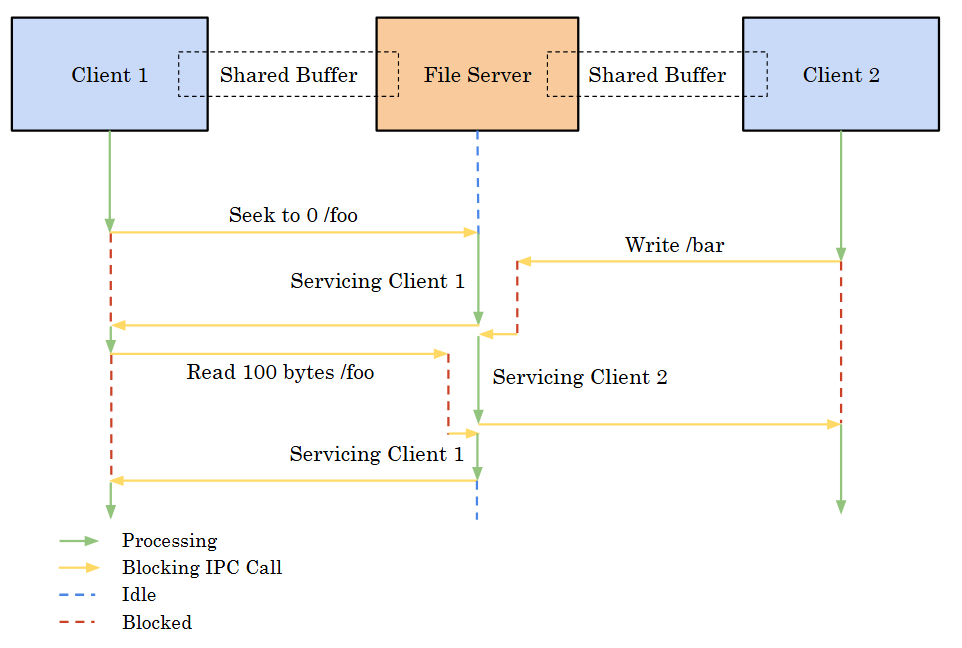
\includegraphics[width=0.6\linewidth]{chapters/images/sync.png}
    \caption{Synchronous multiclient-server interaction.}
    \label{fig:sync}
\end{figure}

Consequently, this model permits no concurrency in relation to the file server, and clients spend a significant portion of time blocked, particularly as the number of clients increases. Additionally, IPC overhead is incurred on a per-operation basis, as each request requires a dedicated interaction with the server. This makes it unsuitable for workloads where large numbers of independent operations are performed, but provides a clear and well-defined baseline for comparison with the asynchronous design.

\subsection{Asynchronous Model \textit{(Proposed IPC Mitigation Strategy)}}\label{sec:ipc_design}

The asynchronous model replaces the synchronous request–response interaction with a non-blocking, decoupled communication approach. While this increases the complexity of the interaction and the resources required, it enables significantly greater potential for performance improvement.

This non-blocking communication is achieved through a notification-based mechanism, rather than procedure calls. As a result, there is no requirement for a handshake or immediate response, allowing the client to issue a notification and continue execution without blocking, as illustrated by the continuous client execution in Figure~\ref{fig:async}. However, if the following computation relies upon the result of the requested operation, and no later processing may be moved forwards, the client will still have to wait. Yet, this model provides flexibility, enabling concurrency where possible while preserving correctness when dependencies exist.

When the server is idle, a notification triggers immediate processing of the corresponding request. Otherwise, unlike the synchronous system, where clients wait until the server becomes available to transfer their request, request submissions must be stored until they can be processed. As the server may be busy, this queuing cannot be managed internally by the server at the time of submission. Instead, each client is assigned a dedicated shared memory region with the server, used to queue outstanding requests. Notifications therefore carry no data, acting solely to signal that work is available, while the actual request data is retrieved by the server from these shared memory queues. As such, upon completing an operation the server polls these client queues to identify and service any pending requests that may have been submitted while it was busy.

To support efficient and correct operation, this shared memory must be carefully structured. As in the synchronous design, a separation between operation metadata and operation data is maintained. However, due to the absence of message-based data transfer, a queue of submission entries is required in addition to per-operation data buffers. To enable multiple outstanding requests without contention, a pool of submission buffers is used rather than a single shared buffer. This pool must be bounded to balance memory usage against achievable concurrency. Therefore, alongside the necessary metadata, each submission entry must include a reference to the operations associated buffer.

A corresponding completion queue and set of response buffers are provided for the server to return results. Separating submission and completion structures avoids the need for in-place modification of request data, which simplifies reasoning about ownership and correctness. This design ensures that each buffer has a clear single producer – single consumer relationship, reducing the risk of data corruption, and avoiding unnecessary allocation of buffers for operations that do not require them.
 \newpage
As operations are completed in-order per client, completion entries correspond directly to submitted operations, allowing the client to match responses to their original requests. To acquire these responses, a client may either poll the completion queue or wait for a notification from the server indicating that results are available. Each completion entry then contains the result of the operation, including any return value or error status, as well as an optional response buffer index, allowing the client to determine whether the request was successful.

By decoupling request submission from notification, this design implicitly enables batching. A client may enqueue multiple requests before notifying the server, allowing a single IPC event to trigger the processing of multiple operations. This reduces the number of IPC interactions required and amortises communication overhead across a batch, as illustrated by Client~1 in Figure~\ref{fig:async}. To maximise efficiency, the server processes all queued requests for a client before polling others. However, this must be bounded to prevent starvation, ensuring fair servicing across clients. To maintain correctness, queue entries are marked as ready explicitly by the client, rather than relying solely on queue occupancy, allowing the server to distinguish between valid and incomplete submissions.

%  TODO vspace
\begin{figure}[H]
    \centering 
    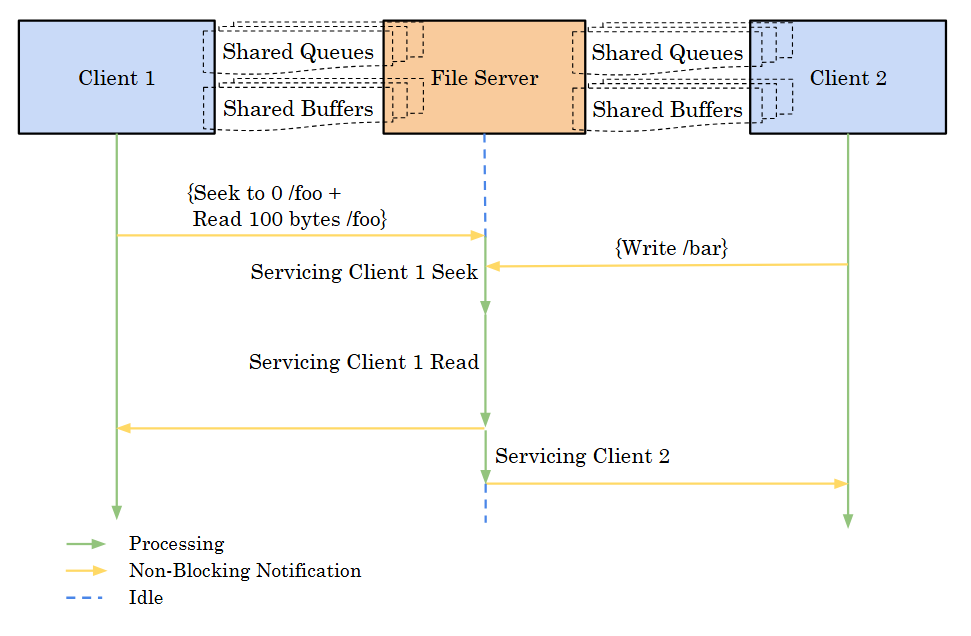
\includegraphics[width=0.68\linewidth]{chapters/images/async.png}
    \caption{Asynchronous multiclient-server interaction.}
    \label{fig:async}
\end{figure} 

While batching can increase the latency of individual operations, it reduces overall IPC frequency and context switching, significantly improving system throughput. Furthermore, the decoupled nature of the interaction allows client execution and server processing to overlap where possible, reducing unnecessary serialization and enabling more efficient utilisation of system resources.

The improvements can be understood through an analytical model of the system. Let $a_n$ denote the time taken for a batch of $n$ operations in the asynchronous system, then let $x$ represent the internal processing time per operation and $c_{a_n}$ represent the communication overhead for the batch.

Therefore, the total execution time for an asynchronous batch of operations can be expressed as:

\begin{equation}
a_n = c_{a_n} + n x
\end{equation}

Hence, the average time per operation is:

\begin{equation}
\frac{a_n}{n} = \frac{c_{a_n}}{n} + x
\end{equation}

This shows that as the batch size increases, the communication overhead is amortised across multiple operations, causing the per-operation communication cost $\frac{c_{a_n}}{n}$ to decrease. In the limit, the average operation time approaches the internal processing cost $x$, indicating that communication overhead becomes negligible.

This highlights the fundamental advantage of batching, as it allows the system to approach a performance bound determined primarily by computation rather than communication.

\section{File Server}

The following subsections discuss the internal design of the file system, including its data structures and organisation. The design focuses on providing a simple and efficient structure to support the required operations, while remaining compatible with both synchronous and asynchronous interface models. 

\subsection{Architectural Overview}

The file server is structured as a set of modular components, each responsible for a distinct aspect of file system operation. Rather than treating the server as a single monolithic body of logic, functionality is decomposed into separate components for request handling, file system operations, runtime state management and storage management. Together, these provide a unified file system service to clients while maintaining clear internal separation of concerns, in keeping with core microkernel design principles.  Furthermore, this modularity supports uniform error handling, allowing failures to be detected accurately, propagated naturally between components and returned to clients in a consistent manner.

At the highest level, the request handling layer forms the entry point into the server, receiving operations from clients and dispatching them to the appropriate file system logic. The file system core implements the semantics of individual file operations, coordinating access to the internal data structures required to service them. Runtime state management maintains transient execution state associated with active file handles, such as access modes and file offsets, while the storage management layer manages the underlying in-memory representation of file contents, metadata and allocation state. This decomposition is illustrated in Figure~\ref{fig:arch}.
\newpage

\begin{figure}[H]
    \centering
    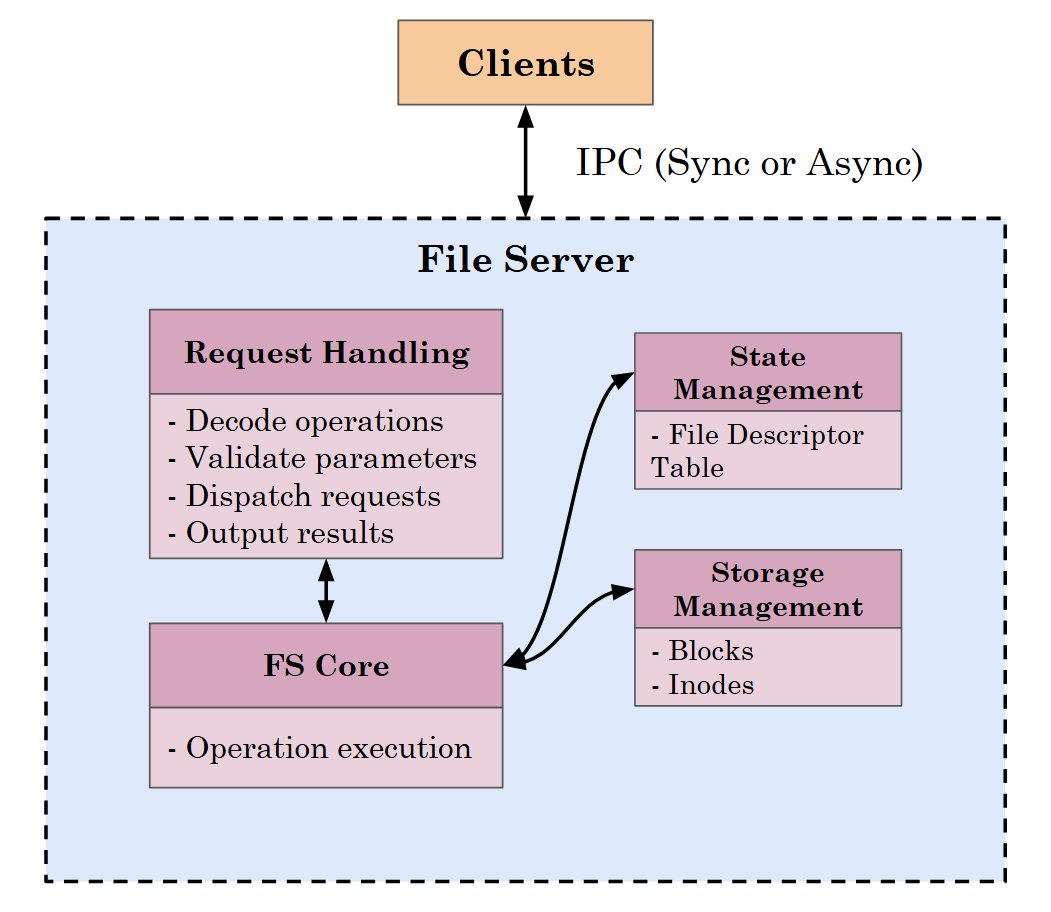
\includegraphics[width=0.55\linewidth]{chapters/images/arch.png}
    \caption{Architectural overview of the file server.}
    \label{fig:arch}
\end{figure}

At a system level, the file server is responsible for servicing client file operations, maintaining correctness of file system state, managing storage resources, and coordinating access across multiple clients. Importantly, these responsibilities are independent of whether requests arrive through the synchronous or asynchronous interface, as both models share the same internal file system logic. This ensures that differences in measured performance arise from interface behaviour rather than differences in core file system operation.

This modular structure allows internal structures or algorithms to be modified without affecting the overall architecture, while supporting extensibility, as features such as persistent storage, more advanced allocation schemes or alternative caching strategies could be introduced without fundamentally redesigning the server.

Hierarchical file storage through a directory structure is supported, allowing files and directories to be organised using path-based naming. Directories may contain both files and subdirectories, enabling nested storage and traversal in a conventional tree-like structure. This was chosen over a flat namespace to support structured organisation and realistic file system behaviour. 

The file server supports a set of operations intended to provide a sufficiently complete and practical file system interface for both functional use and evaluation. These include file and directory creation (Create File, Create Directory), data access (Read, Write, Seek), file lifecycle management (Open, Close, Delete), metadata and state queries (Get Size, Exists, Get Permissions, Set Permissions), and directory enumeration (List).

This set was chosen to provide a balanced interface spanning namespace management, data access, runtime file state and metadata handling. Together, these operations exercise the principal structures and responsibilities of the file server without introducing unnecessary complexity beyond the scope of this work.

\subsection{Component Design and Interactions}

Significant storage management is required to support file system operations, motivating separate structures for representing data, metadata, runtime state and namespace organisation, along with mechanisms to govern their interaction. 

\subsubsection{Blocks}

Blocks form the fundamental unit of data storage in the file server. They represent fixed-size regions of memory used flexibly to hold dynamic file system data, including file contents, directory entries and, where required, block indices for indirect blocks. Using a unified block abstraction allows storage to be allocated according to demand, rather than partitioning memory into separate fixed regions for different data types. This provides greater flexibility, allowing files and directories to grow as required while also avoiding unnecessary reservation of space when demand is low.

A fixed block size was chosen to simplify allocation, indexing and data extension. A size of 4~KiB was selected as a practical balance between storage granularity and management overhead. While fixed-size allocation means all operations occur at block granularity, potentially wasting space when storing very small files, this was accepted in exchange for more efficient allocation management and simpler indexing. As the system is modular, however, this block size remains configurable.

Blocks are managed through an block allocation table, as illustrated in Figure~\ref{fig:bat}. This maintains one entry per block, with each entry storing a flag indicating whether the corresponding block is free or allocated. This enables rapid assignment and release of blocks, simplifying rearrangement of file system data.

\begin{figure}[H]
    \centering
    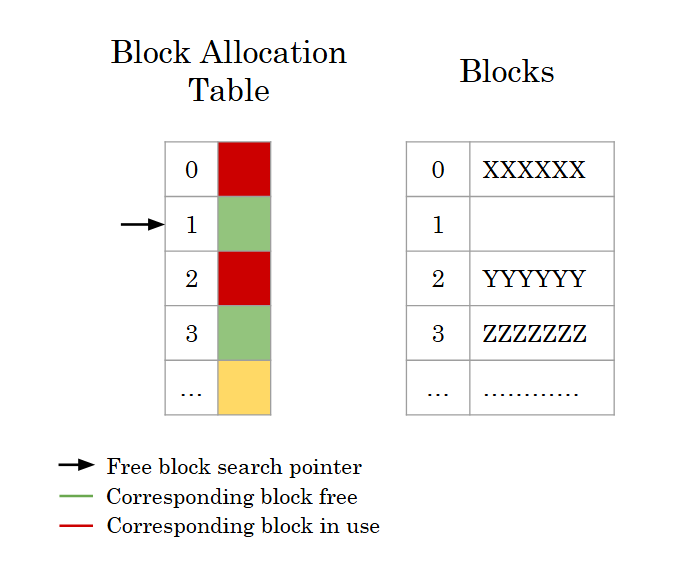
\includegraphics[width=0.55\linewidth]{chapters/images/block_alloc.png}
    \caption{Block allocation table structure.}
    \label{fig:bat}
\end{figure}

All blocks are stored contiguously and are accessed by index into the block pool, with these indices being stored within inodes.

\subsubsection{inodes}

Inodes provide the central metadata structure of the file system, representing either files or directories and linking their logical identity to the underlying storage by holding both entry metadata and block references. This structure was chosen to separate metadata from data storage, simplifying management of file system state. It also provides a uniform representation for file system objects, reducing special-case handling. Furthermore, resolving persistent objects independently of their names avoids repeated path-based lookup. 

\begin{figure}[H]
    \centering
    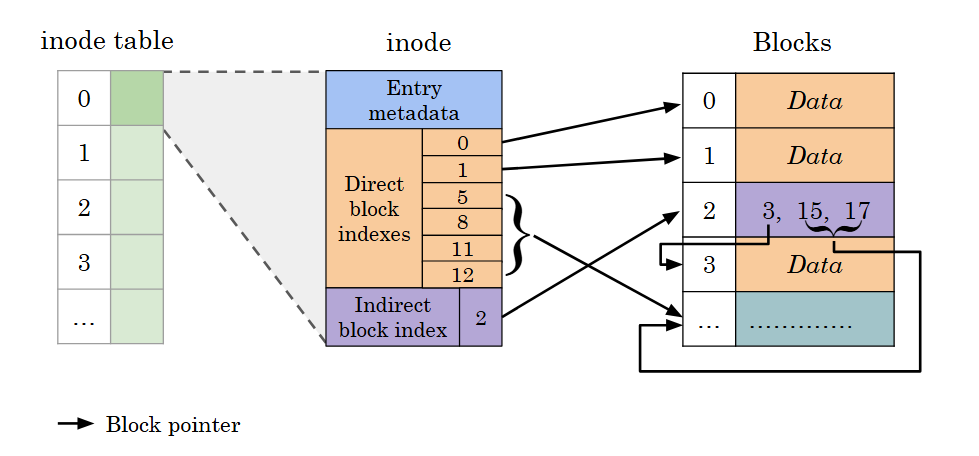
\includegraphics[width=0.8\linewidth]{chapters/images/inode.png}
    \caption{inode and block reference structure.}
    \label{fig:indirect-blocks}
\end{figure}

This metadata must hold a variety of information to allow rich and secure system functionality. To avoid requiring a separate allocation table, each inode includes an in-use flag to enable rapid allocation and deallocation. The inode type (file or directory) is also stored, ensuring associated data is interpreted appropriately and supporting valid file traversal. Ownership and access permissions are additionally stored to support multiple clients safely. 

Inodes store block references either directly or, where additional references are required, through indirect blocks, as shown in Figure~\ref{fig:indirect-blocks}. This allows files to grow beyond the capacity of direct block references while preserving a uniform access model, although very large files may incur modest additional access overhead due to indirect reference resolution. 

To aid efficient data access and ensure only initialised storage is accessed, an inode also stores the file size, indicating the extent of valid file data. Together with the block references, this supports Read operations through resolution of valid file data and Write operations through access to existing blocks, while determining when file extension requires allocation of additional blocks. 

This design introduces an additional level of indirection between file system objects and their underlying data, but this was accepted in exchange for the flexibility, uniformity and scalability the inode structure provides. 

\subsubsection{Directories}

Directories provide the namespace structure of the file system, enabling hierarchical organisation through mappings from names to inode references. They are represented using the same inode and block structures used elsewhere in the file system, reusing existing abstractions rather than requiring a separate storage mechanism, thereby preserving flexibility in data use and storage efficiency. 
\vspace{0.3cm}
\begin{figure}[H]
    \centering
    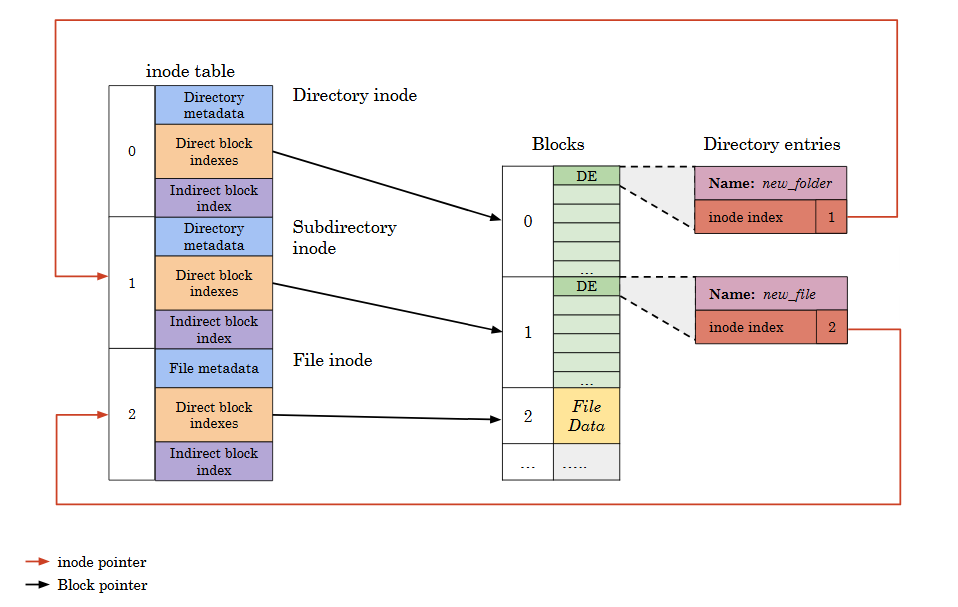
\includegraphics[width=0.9\linewidth]{chapters/images/dir_inode.png}
    \caption{Directory structure via inodes and blocks.}
    \label{fig:directory-entries}
\end{figure}

A directory is represented by a directory inode whose associated blocks store a list of nested files and subdirectories as directory entries. Each directory entry is a structure linking an entry name to its respective inode via an index, as shown in Figure~\ref{fig:directory-entries}. 
\newpage
This recursive structure enables hierarchical namespace organisation through arbitrary nesting of directories and files, supporting structured management beyond what would be possible in a flat namespace. It also provides inherent path-based access, where successive path segments are resolved by searching the entries of the current directory, descending into a child directory when a matching entry is found, until the target inode is reached, or a path is deemed invalid. This traversal mechanism is used by file system operations to inspect and modify directory entries, enabling Create to enforce valid paths and prevent duplicate names within a directory, while supporting recursive directory deletion through traversal of all contained entries to ensure no unreachable data is left allocated. 

For general use, a root directory is created during system initialisation, through which all files and directories are organised upon, hence, may not be deleted. Special directory entries such as . and .., as well as symbolic links, are not supported, reducing namespace complexity and avoiding additional traversal cases. 

This structure was chosen to support path-based access and structured file lookup, allowing files to be located through traversal rather than requiring a flat naming model. However, as path resolution requires directory traversal, lookup incurs some overhead, particularly due to linear directory scans and possibly deeply nested paths. Linear scanning was chosen over more complex indexed lookup structures to reduce management overhead and implementation complexity, which was considered appropriate for the expected scale of the file system, while not affecting comparisons of the synchronous and asynchronous communication models. 

\subsubsection{File Descriptors}

File descriptors maintain runtime state for open files, providing a layer of indirection between client operations and persistent file metadata. As shown in Figure~\ref{fig:file-descriptors}, a file descriptor links a client-visible handle to the inode representing the underlying file, while additionally storing the transient state required for continued access.

\begin{figure}[H]
    \centering
    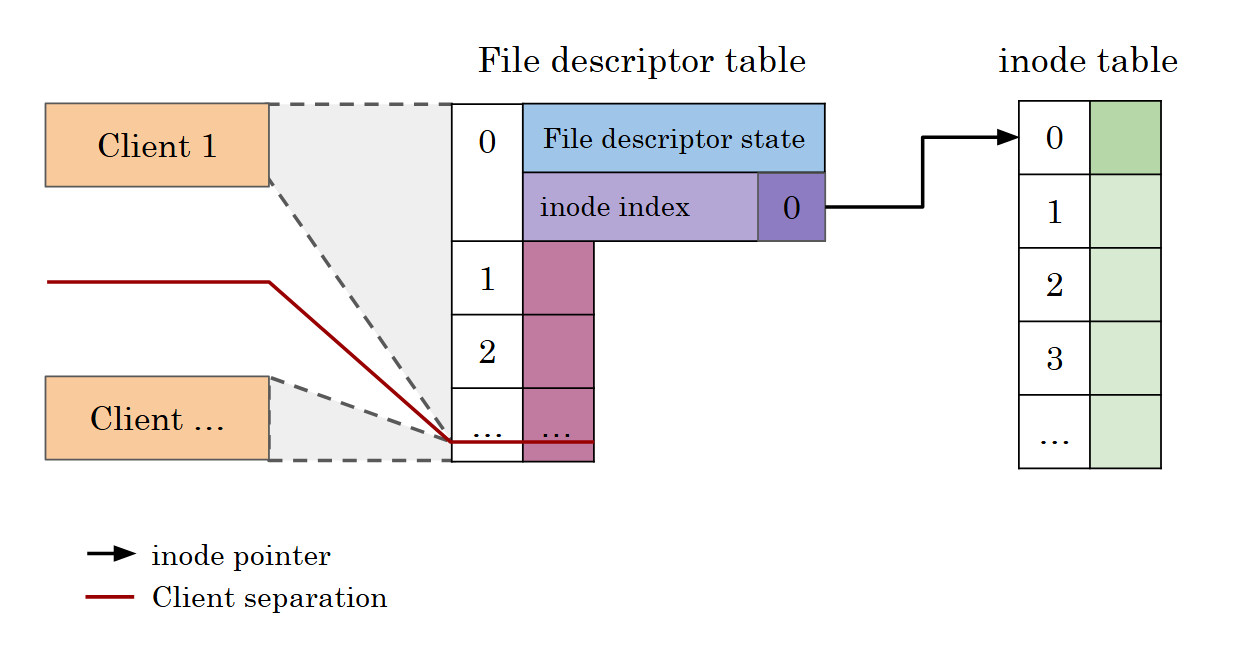
\includegraphics[width=0.7\linewidth]{chapters/images/fds.png}
    \caption{File descriptor structure.}
    \label{fig:file-descriptors}
\end{figure}
\newpage

This state includes a reference to the associated inode, the current file offset, and the mode in which the file was opened. Separating this runtime state from inode metadata allows information specific to an active open instance, rather than the file itself, to be maintained, supporting multiclient access. This is additionally useful for operations such as sequential reads or writes, where file position may persist across operations and need not be re-specified.

File descriptors are created and returned to a client when a file is opened, and are subsequently used by operations such as Read, Write, Seek and Close to reference the open file. This improves efficiency by avoiding path resolution for every operation, as the file descriptor is used to link directly to the associated inode.

This design does introduce some overhead in maintaining descriptor state, but this is modest relative to the performance benefits it provides. Fixed-size file descriptor regions do, however, impose a bounded number of simultaneously open files per client.

\subsection{Request Processing Flow}

File system requests follow a common processing path regardless of operation type. Once a request is received by the file server, it is first decoded to determine the requested operation and extract any associated parameters. Basic validation is then performed, such as verifying the operation code is recognised, the required parameters are present and checking that any referenced file handles or paths are correctly formed.

Following validation, the request is dispatched to the appropriate file system logic. Although the specific structures accessed differ by operation, all requests follow the same general pattern of interacting with the file system core, consulting or updating the relevant runtime state, accessing the underlying storage structures as required, and generating a result to return to the client.

The general flow is:
\begin{itemize}
    \item Receive request
    \item Decode operation
    \item Validate parameters
    \item Service operation
    \item Access internal structures
    \item Update state if required
    \item Generate response
\end{itemize}

For example, Read request follows this general structure by validating the supplied file handle exists and is a file, consulting the open file state to determine the current offset, resolving the relevant storage blocks containing the requested data, and returning the result while updating the file offset. Operations such as Create and Write access and modify different state, but follow the same overall dispatch and servicing model.

This shared processing path was chosen to reduce duplicated logic, ensure consistent validation across operations, and simplify reasoning about correctness within the file server.

\subsection{Multiclient Support}

Multiclient support is provided through a combination of per-client runtime state, client isolation and centralised coordination through the file server. This allows multiple clients to access the file system concurrently while preserving correct behaviour and separation of client context.

Per-client state is maintained through both persistent and runtime structures. Ownership and access permissions are stored within inode metadata, allowing access control decisions to be enforced consistently regardless of which client issues a request. Permissions are represented using read, write and execute flags, allowing the file server to determine whether a client may perform a requested operation. Ownership associates each file or directory with the client that created it and restricts operations such as permission modification. Ownership also supports private access: if a permission flag is unset, only the owner may perform the corresponding operation, whereas if the flag is set, any client may do so. 

Runtime state associated with open files, such as file offsets and access modes, is maintained in file descriptors. To preserve client independence, each client is assigned a separate region of the file descriptor table, with a local maximum number of open files. This ensures that one client’s open file state cannot interfere with that of another. This separation of runtime state provides client isolation even when multiple clients access shared resources. While multiple clients may access the same underlying file, each does so through its own client context, maintaining independent offsets, access modes and descriptor state.

Consistency of shared resources is preserved through centralised mediation by the file server; all file operations pass through the server and are serviced atomically, with updates to shared file system structures serialised. 

A particular case of shared resource consistency arises when one client deletes a file that remains open by others. In this case, deletion is deferred until the final client closes the file, ensuring that active references remain valid and preventing removal of data still in use.


\chapter{Implementation}
\label{cha:implementation}


\section{Development Environment and Tools}

The system was implemented in C using the Microkit framework for seL4, specifically version 2.0.1 of the Microkit SDK\cite{}. Development targeted the AArch64 architecture\cite{}, with code compiled using the aarch64-linux-gnu cross-compilation toolchain. The build process was managed using a Make-based system, which coordinated compilation, linking and generation of Microkit system images.

All development and testing were conducted in an emulated environment using QEMU\cite{}, targeting the virt platform with a Cortex-A53 CPU configuration. This allowed rapid iteration without requiring physical hardware, though it limits evaluation of hardware-specific performance characteristics.

Debugging and verification were primarily performed using logging via serial output, enabling inspection of system behaviour during execution. Additional support tools included Git\cite{} for version control and reproducibility of development progress.

\section{Microkit Framework Setup}

The system is built using the Microkit framework for the seL4, which provides a declarative mechanism for defining system structure, memory layout and inter-process communication\cite{}. A Microkit system is specified using an XML-based description, which is used to generate a complete system image comprising multiple protection domains.

Each protection domain represents an independent user-space process with its own address space and execution context. In this system, separate protection domains are defined for the file server and each client. Program images are statically assigned to each domain, and memory regions are explicitly declared and mapped into their address spaces at specified addresses. A dedicated memory region for file system state is declared and mapped solely to the server. Additionally, for each client, regions to hold submission and completion queues and associated buffers are declared and mapped into both the file server and the corresponding client, each with the appropriate permissions, allowing shared access.

Alongside this shared memory, communication between protection domains is established using channels, which define endpoints for inter-process communication, with each client being connected to the file server. For the synchronous system, protected procedure calls\cite{} are used to perform synchronous message passing to request file operations and block until a response is received. In contrast, the asynchronous design utilises notification objects\cite{}, which provide non-blocking signalling to indicate when requests have been submitted or responses are available.

As Microkit systems are statically defined, the number of clients and their associated resources must be specified at build time. To support varying workloads, a script was developed to automatically generate the system description for a configurable number of clients, ensuring consistency while avoiding manual duplication.

In addition to structural configuration, Microkit also requires specification of priority and scheduling parameters for each protection domain. These priorities determine the order in which domains are scheduled by the seL4 kernel, directly influencing system responsiveness and fairness. In this system, the file server is assigned a higher priority than client domains to ensure that incoming requests are serviced promptly, reducing queuing latency and preventing clients from stalling due to delayed processing. Client domains are assigned equal priorities relative to one another to maintain fairness across request sources. This scheduling configuration is particularly important in the asynchronous design, where the server must efficiently respond to notifications and process queued operations without being preempted excessively. Consequently, as seL4 utilises a round-robin style scheduling policy\cite{}, careful time budget allocation ensures that IPC handling remains responsive while still allowing clients sufficient execution time to generate and consume requests.

\section{Interface}
\subsection{Synchronous Server Model}
\subsubsection{Client-Server Communication Protocol}
\subsubsection{IPC Mechanism}
\subsubsection{API}
\subsection{Asynchronous Server Model}
\subsubsection{Client-Server Communication Protocol}
\subsubsection{IPC Mechanism}
\subsubsection{API}

\section{File Server}
\subsection{Data Structures and Access Methods}
\subsubsection{inodes}
lorem
\subsubsection{Blocks}
\subsubsection{Directories}
\subsubsection{File Descriptors}

\subsection{Operations}
\subsubsection{Entry Creation}
\subsubsection{File Access}
\subsubsection{Metadata Access and Modification}
\subsubsection{Entry Deletion}

\section{Error Handling}

The primary sources of errors in this system arise from invalid client requests and resource limitations. These include cases such as invalid permissions, malformed paths or file descriptors, as well as exhaustion of resources such as available blocks or file descriptor space. To maintain correctness, these conditions are explicitly checked before and during the execution of each operation.

To support this, operations are decomposed into smaller functions, each responsible for a specific task. At each potential point of failure, inputs and system state are validated, with failures resulting in the return of a defined error code from a global set. These error codes are propagated through the call chain, allowing higher-level operations to respond appropriately. Where possible, alternative actions are attempted; otherwise, the operation is safely terminated, reverting any partial changes to maintain consistency. The final error state is then communicated back to the client through the response structure. Some errors such as trying to read a size larger than the buffer size do not terminate the operation, but the client is still notified that it was not fully successful.

\chapter{Evaluation}
\label{cha:evaluation}


\section{Validation}

Extensive validation was conducted to ensure the correctness, robustness and reliability of the file server under both normal and adverse conditions. Given the range of supported operations, numerous edge cases and error scenarios arise. Additionally, the presence of multiple clients and asynchronous communication introduces further complexity, requiring testing not only to verify functional correctness but also to ensure that the system maintains consistency and stability under concurrent workloads.

To increase confidence in the correctness of the system as a whole, testing was conducted at multiple levels. Initially, unit testing was used to verify the functionality of individual components in isolation. This enabled a modular development approach, allowing components to be validated incrementally during implementation. Testing at this level also simplified debugging, as errors were easier to localise due to their limited scope and the reduced code surface. 

However, as the system relies heavily on interactions between components and communication between protection domains, integration testing was also necessary. This enabled validation of end-to-end behaviour, ensuring that all operations functioned correctly when executed through the full client–server interface under a range of conditions.

\subsection{Unit Tests}

Unit tests were developed for the core of the file system, including components such as block management, inode management, directory handling and file table operations. These tests focused solely on verifying the correctness of the file server’s data structures and their accesses.

To ensure this isolation, these components were tested by directly invoking their functions outside of the Microkit environment. This allowed inputs and supporting data to be mocked through deterministic flows, and the internal state of the file system to be inspected, enabling correctness to be validated at each stage of execution. Testing regular inputs alongside failure conditions such as resource exhaustion gave confidence that the fundamental building blocks of the file system operated correctly before integration and would not cause wider issues upon failure.
\newpage
For example, one test constructs a mock “indirect block” containing a list of allocated block indices, invokes the indirect-release routine, and then verifies that each referenced block is marked free in the allocation table.


\subsection{Integration Tests}

Once the components were verified, integration testing was used to validate the behaviour of the system as a whole, exercising all file system operations through its regular running microkit environment. Rather than directly inspecting internal state, validation was performed through the responses and error codes returned to clients, such as creating a file then listing the file system. This ensured that testing reflected real system usage and confirmed that correct behaviour was exposed through the public interface.

\subsubsection{Single Client}

These tests exercised the majority of functionality from the client’s perspective, covering the full lifecycle of files, including creation, reading, writing and deletion, without the added complexity of concurrent access. Within this scope, it was possible to verify that invalid client inputs were correctly rejected with appropriate error codes, for example when attempting to delete a non-existent file. Additionally, boundary conditions were tested to ensure correct behaviour under extreme cases, such as reading the maximum supported amount of data.

\subsubsection{Multiple Clients}

To ensure that all clients were serviced correctly and fairly, and that the system operated reliably under load, extended tests were conducted which interleaved operations from multiple clients. This enabled validation of scenarios that cannot be observed in a single-client context, including permission enforcement and modification of shared resources.

As clients execute independently, explicit synchronisation was required. This was achieved through the use of marker files, where clients created files with predefined names that were monitored by other clients. These acted as barriers, allowing coordination of execution order and enabling clients to signal completion of operations to both the server and one another. For example, one test creates a publicly readable file within client 1, after which client 2 attempts to read the file to verify access is permitted. The file is then modified by client 1 to be private, and client 2 subsequently attempts to read it again, verifying that the operation is correctly rejected with a permissions error.

\section{Performance Evaluation}

\subsection{Goals}

The primary goal of this evaluation was to compare the performance characteristics of the synchronous and asynchronous file server designs. In particular, the evaluation aimed to quantify the impact of inter-process communication (IPC) overhead and assess the effectiveness of batching in reducing per-operation cost. Additionally, the behaviour of both systems under multiclient workloads was examined to determine how well each design scales under contention.

\subsection{Metrics}

For the per operation benchmarking, performance was evaluated using the average time per operation, calculated by measuring the total execution time of a long sequence of operations, to amortise any stochastic effects, and dividing by the number of operations performed. For the more realistic workflows, time taken to complete the whole suite was used. These provided consistent bases for comparing synchronous and asynchronous implementations.

Time measurement was performed using the CPU cycle counter, as the low-level execution environment does not provide native timing facilities. The cycle count was recorded before and after each client’s measurable operations, and converted to elapsed time using the processor’s clock frequency. Results were averaged across multiple runs to reduce variance and improve reliability.

In multiclient scenarios, fairness was also considered. This was validated by recording the total time taken by each client to complete its workload, ensuring that no individual client experienced disproportionate delay.

\subsection{Experimental Setup}

All experiments were conducted within the same emulated environment using QEMU on an AArch64 platform, ensuring consistency across all tests. Both synchronous and asynchronous implementations were evaluated under identical conditions, with the same workloads, file sizes and file system state.

For each experiment, the only variables altered were the server design (synchronous or asynchronous), the batching configuration and the number of clients. All operations were validated for correctness during execution to ensure that performance results reflected valid system behaviour rather than erroneous outcomes. During the varied workload, this processing also mimicked non-file I/O that would occur in a typical system, helping to ensure that the measured performance reflects realistic operating conditions.

\subsection{Benchmark Design}

Two benchmark suites were developed to evaluate system performance. The first was designed to isolate and quantify the reduction in communication overhead achieved by the asynchronous server, while the second evaluated overall system performance under more realistic and varied workloads.

This initial aim was achieved through a single-client benchmark that repeatedly executed a single type of operation allowing controlled measurements of individual operation costs for both systems. Both read and write operations were evaluated independently, as they are representative of common file system usage and exhibit differing behaviour. As timing was recorded from the client’s perspective, this included both internal server processing time and communication overhead.

For the asynchronous implementation, the benchmark was executed with varying batch sizes. A batch size of one provided a baseline comparison, ensuring that the asynchronous design does not significantly degrade performance when batching is not possible, which is important as many real workloads contain inherent dependencies. Larger batch sizes allowed evaluation of how batching reduces per-operation cost, identifying the point at which performance improvements become significant and where further increases yield diminishing returns.

As the internal file system operation of both systems are the same, this benchmark also enabled estimation of communication overhead. Let $s$ denote the time taken for a single operation in the synchronous system and $a_n$ the time taken for a batch of $n$ operations in the asynchronous system. Let $x$ represent the internal processing time per operation, and $c_s$ and $c_{a_n}$ the communication overheads. Then:

\begin{equation}
s = c_s + x
\end{equation}

\begin{equation}
a_n = c_{a_n} + n x
\end{equation}

And

\begin{equation}
s \cdot n = c_s \cdot n + n x
\end{equation}

Hence

\begin{equation}
s \cdot n - a_n = c_s \cdot n - c_{a_n}
\end{equation}

Using measured values of $s$ and $a_n$, this relationship allows the difference in communication overhead between the synchronous and asynchronous systems to be quantified across varying batch sizes.

Furthermore:

\begin{equation}
\frac{a_n}{n} = \frac{c_{a_n}}{n} + x
\end{equation}

This formulation also allows analysis of the average cost per operation in the asynchronous system. As the batch size increases, the communication overhead is amortised across multiple operations, causing the per-operation communication cost to decrease. In the limit, the average operation time approaches the internal processing time $x$, indicating that communication overhead becomes negligible. This highlights the fundamental advantage of batching, as it allows the system to approach optimal performance bounded only by computation.

The second benchmark was a multiclient, realistic workload designed to simulate typical file system usage. Multiple clients executed independently, each performing a sequence of  varied operations across many files. This sequence consisted of CREATE, WRITE, CLOSE, OPEN, SEEK, READ and DELETE operations, representing a complete file lifecycle. Operations were interleaved across clients to introduce contention and better reflect real-world usage patterns.

As batching is central to the performance benefits of the asynchronous design, this benchmark was structured to allow batching where it would naturally occur, without artificially constraining the workload. While it is possible to construct workloads with strict dependencies between operations, this would reduce asynchronous behaviour to that of the synchronous system and provide limited insight beyond the single-operation benchmark. Instead, operations were grouped into realistic batches, for example: CREATE | WRITE and CLOSE | OPEN | SEEK and READ and DELETE.

Performance was measured across varying numbers of clients, enabling analysis of scalability, contention and the impact of concurrent access. This approach provided a balanced evaluation, allowing direct comparison of synchronous and asynchronous designs under both controlled and realistic conditions.

\subsection{Results and Analysis}

\subsubsection{Single-Client Per-Operation Benchmark}

\begin{figure}[H]
    \centering
    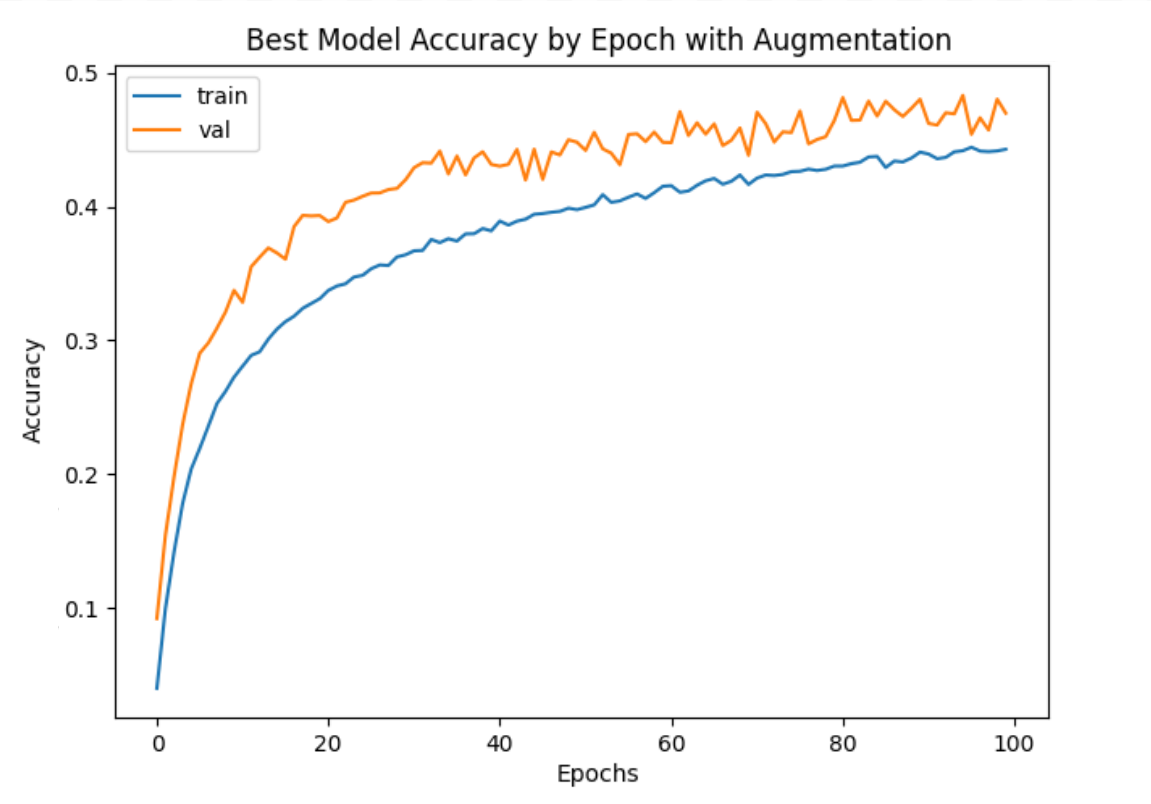
\includegraphics[width=0.7\linewidth]{chapters/images/single_graph.png}
    \caption{Average Time per Operation vs Batch Size (Read and Write)}
    \label{fig:example}
\end{figure}

The synchronous baseline establishes the per-operation cost of IPC without batching. Write operations averaged 186~$\mu$s, while read operations averaged 155~$\mu$s, reflecting the expected asymmetry due to additional data movement and persistence overhead in writes.

When the asynchronous system is configured with a batch size of one, performance is effectively equivalent to the synchronous implementation. Writes measured 187~$\mu$s and reads 158~$\mu$s, indicating that the introduction of asynchronous infrastructure does not impose significant additional overhead in the absence of batching. This validates the design goal that the asynchronous system should degrade gracefully to synchronous-like behaviour when batching is not possible.

As batch size increases, a clear and substantial reduction in per-operation cost is observed. For write operations, the average latency decreases from 187~$\mu$s (batch~=~1) to 74~$\mu$s (batch~=~10), representing approximately a 60\% reduction. Similarly, read operations decrease from 158~$\mu$s to 41--48~$\mu$s, corresponding to a $\sim$70--74\% reduction at optimal batch sizes.

The results exhibit a diminishing returns pattern. The most significant improvements occur between batch sizes 1 and 4:
\begin{itemize}
    \item Write latency drops from 187~$\mu$s to 91~$\mu$s ($\sim$51\% reduction)
    \item Read latency drops from 158~$\mu$s to 63~$\mu$s ($\sim$60\% reduction)
\end{itemize}

Beyond this point, gains become incremental. For example, increasing batch size from 8 to 10 yields negligible improvement for writes (74~$\mu$s $\rightarrow$ 74~$\mu$s) and even slight regression for reads (41~$\mu$s $\rightarrow$ 48~$\mu$s), likely due to increased queuing delay or cache effects.

These results align closely with the analytical model:

\[
\frac{a_n}{n} = \frac{c_{a_n}}{n} + x
\]

As $n$ increases, the amortised communication cost $\frac{c_{a_n}}{n}$ diminishes, and the average operation time approaches the internal processing cost $x$. Empirically, the asymptotic region appears around batch sizes 7--9, suggesting that beyond this range, IPC overhead becomes a minor component of total latency.

Using the relationship:

\[
s \cdot n - a_n = c_s \cdot n - c_{a_n}
\]

we can infer that the synchronous system incurs a linear growth in communication overhead with respect to operation count, whereas the asynchronous system effectively flattens this growth. The widening gap between $s \cdot n$ and $a_n$ as $n$ increases directly quantifies the reduction in IPC overhead achieved through batching.

Notably, read operations benefit more significantly from batching than writes. This suggests that read operations are more heavily dominated by IPC overhead in the synchronous system, whereas writes retain a larger proportion of intrinsic processing cost.

\subsubsection{Multiclient Realistic Workload}

\begin{figure}[H]
    \centering
    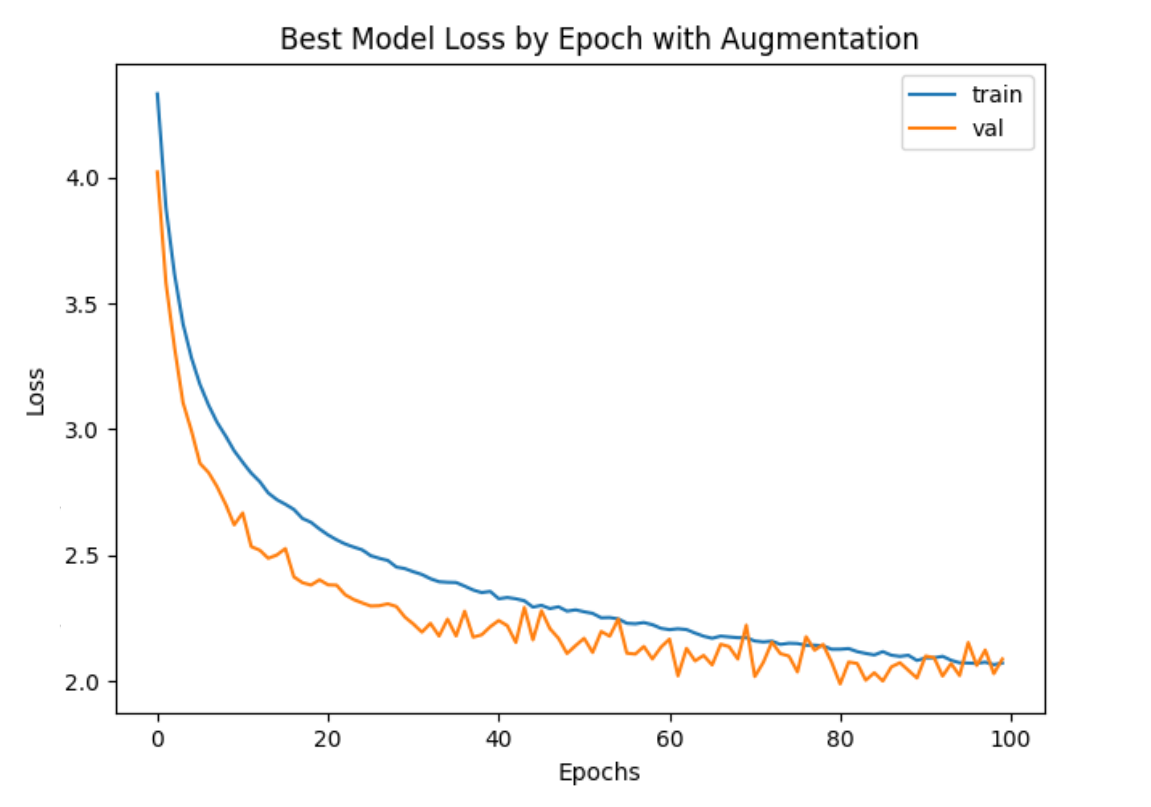
\includegraphics[width=0.7\linewidth]{chapters/images/multi_graph.png}
    \caption{Total Execution Time by Number of Clients (Synchronous vs Asynchronous)}
    \label{fig:example}
\end{figure}

\begin{figure}[H]
    \centering
    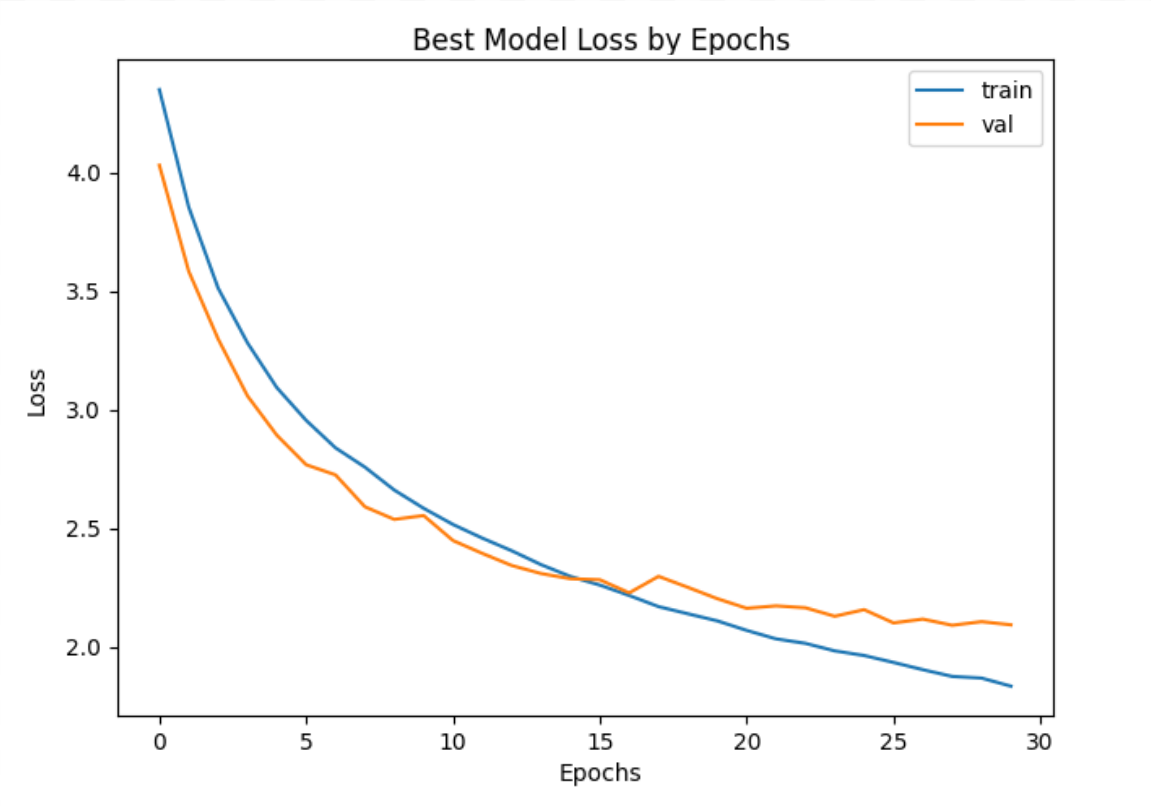
\includegraphics[width=0.7\linewidth]{chapters/images/fairness_graph.png}
    \caption{Execution Times per Client (Fairness Analysis)}
    \label{fig:example}
\end{figure}

Under multiclient workloads, the asynchronous design demonstrates a substantial performance advantage. The synchronous system exhibits total execution times clustered tightly around 25.3--25.7 million~$\mu$s, with per-client averages between 12{,}680--12{,}862~$\mu$s. In contrast, the asynchronous system completes the same workload in approximately 16.0--16.3 million~$\mu$s, with per-client averages between 7{,}844--7{,}941~$\mu$s.

This corresponds to an overall performance improvement of approximately 36--38\%, which is consistent with the reductions observed in the single-operation benchmark when moderate batching is achievable.

Fairness across clients is well maintained in both systems. The variation in per-client average time is minimal:
\begin{itemize}
    \item Synchronous: spread of $\sim$182~$\mu$s ($\sim$1.4\%)
    \item Asynchronous: spread of $\sim$97~$\mu$s ($\sim$1.2\%)
\end{itemize}

This indicates that neither system introduces significant starvation or prioritisation bias. Importantly, the asynchronous design preserves fairness despite its more complex scheduling and batching behaviour.

Another notable observation is the consistency of asynchronous performance across clients. The tighter clustering suggests that batching and concurrent handling smooth out transient delays, reducing sensitivity to contention patterns. In contrast, the synchronous system, while still fair, shows slightly higher variability, likely due to clients serialising on IPC interactions with the server.





\chapter{Conclusion}
\label{cha:conclusion}

This dissertation set out to investigate whether inter-process communication (IPC) overhead in the seL4 microkernel could be mitigated through architectural and interface-level design choices, specifically via an asynchronous, multiclient file server. In doing so, it involved the design and implementation of a complete system, encompassing not only the file server itself but also the surrounding infrastructure required to support client interaction, memory sharing and communication within the Microkit framework. By reducing the number of synchronous interactions and enabling batching and decoupling of requests, the work demonstrates that meaningful performance improvements are achievable even within the constraints of a formally verified microkernel environment.

The results show that IPC overhead is not merely a function of the underlying kernel primitives, but is significantly influenced by higher-level system design decisions, particularly how clients interact with services, how requests are scheduled and processed and how system components are structured to minimise unnecessary communication. Furthermore, the development of a full, working system highlights that such optimisations must be considered holistically, as performance gains emerge from the interaction between interface design, scheduling behaviour and data management rather than from any single component in isolation.

\section{Contributions}
\subsection{System Design and Implementation}

This work presents a complete user-space file server built using the seL4 Microkit framework, designed with both synchronous and asynchronous interfaces. The system supports multiple concurrent clients, a structured file system abstraction and a reasonably comprehensive set of file operations including file data, directory, lifecycle and metadata management.
\newpage
Key contributions include:
\begin{itemize}
    \item A modular file system architecture, that can scale and adapt flexibly through its incorporation of block management, inodes and file descriptors, suitable for microkernel deployment
    \item A multiclient design supporting permission enforcement and organised client state management
    \item Dual interface implementations: a traditional synchronous IPC model and an asynchronous model based on notifications, queues and shared buffers
    \item A flexible API layer enabling transparent, simple use of either communication paradigm
    \item A full implementation within Microkit, demonstrating practical use of channels, notifications, scheduling and memory management
\end{itemize}

The implementation validates that complex, stateful services such as file systems can be realised entirely in user space within seL4, while maintaining structured interaction patterns and correctness guarantees.

\subsection{IPC Overhead Mitigation Insights}

The primary analytical contribution lies in demonstrating how asynchronous communication reduces IPC overhead through batching and reduced synchronisation frequency.

The evaluation yields several key insights:
 
\begin{itemize} 
    \item Baseline parity: Asynchronous communication with batch size 1 performs similarly to synchronous IPC, confirming minimal overhead from the abstraction itself
    \item Batching effectiveness: Increasing batch sizes significantly reduces per-operation latency, demonstrating amortisation of IPC costs
    \item Low batch size required for performance maximisation: Performance improvements plateau beyond moderate batch sizes, indicating practical upper bounds for batching efficiency
    \item Workload sensitivity: The benefits of asynchronous IPC are highly dependent on workload characteristics, especially the degree of operation parallelism and batchability
    \item Multiclient scalability: In realistic multiclient scenarios, asynchronous design also substantially reduces average operation latency compared to synchronous approaches
\end{itemize}

These findings reinforce that IPC overhead mitigation is best addressed at the system design level rather than solely through kernel optimisation\cite{}.

\section{Drawbacks and Limitations}

Despite achieving its objectives, the system has several limitations that constrain both performance and general applicability.

\subsection{File System Limitations}

The implemented file system is functionally rich and reasonably well validated, but could be improved in multiple areas. Additional operations such as file renaming and copying could be introduced to improve usability. Furthermore, lookup performance is suboptimal due to linear search mechanisms; the absence of more efficient indexing structures (e.g. hash tables or trees) contributes to increased latency as the file set grows, yet the current implementation is sufficient for general usage and the experiments undertaken in this report.

\subsection{Benchmarking Constraints}

Evaluation required the development of custom benchmarks due to the specialised environment, low-level platform and non-standard interface. While these benchmarks effectively demonstrate relative performance trends, they limit direct comparability with existing systems. Consequently, results should be interpreted as indicative rather than absolute.

\subsection{Lack of Persistent Storage}

The system operates entirely in memory, with no backing disk. Incorporating persistent storage would introduce additional complexity, particularly around buffering strategies, write-back policies and cache management. This would likely require a significantly larger cache and careful coordination between storage and IPC layers, representing a substantial extension beyond the current scope.

As such, the absence of disk I/O results in highly deterministic and relatively low operation latencies. In a realistic system with persistent storage, operation timings would be significantly longer and less deterministic due to device latency, queuing effects and variability in access times. As a result, the relative impact of IPC overhead would be reduced, since communication costs would form a smaller proportion of total operation latency. Consequently, while the results clearly demonstrate IPC-related performance trends, they likely represent an upper bound on the benefits of communication overhead reduction in real-world storage-backed systems. 

However, such systems would typically operate on multi-core hardware, unlike the single-threaded environment used in this work. In these settings, an asynchronous design such as the one presented here, would considerably offset these reduced benefits by enabling significantly higher throughput through concurrent execution.

\subsection{Single-Threaded Execution}

The server operates on a single thread, restricting its ability to exploit concurrency. This inherently limits throughput and reduces the potential benefits of the asynchronous design. In a multi-core system, multiple clients could concurrently issue requests and process responses in parallel with the server executing operations, significantly increasing overall system throughput. In contrast, the synchronous model effectively serialises access, as clients must block and wait while the server processes each request, limiting concurrency at the system level.

The architecture presented here is, however, designed to be transferable to a multicore environment with only minor modifications, once such support is more readily available within seL4.

This limitation also impacts the interpretation of benchmark results. The observed performance improvements arise primarily from reduced communication overhead through asynchronous batching, rather than from true parallel execution. As a result, the measured gains likely represent a conservative estimate of the performance improvements achievable in a fully concurrent system, where additional benefits from overlapping request generation, processing and response handling would be realised.

\subsection{Dependency on Workload Characteristics}

The effectiveness of the asynchronous model is strongly workload-dependent. In scenarios with low concurrency or minimal opportunity for batching, the advantages over synchronous IPC diminish. This indicates that asynchronous designs are not always superior, but instead most effective in systems with naturally parallel or high-throughput workloads.

\subsection{Additional Client Burden}

The asynchronous design introduces additional complexity on the client side, primarily due to the need to manage request queues and response buffers. Each client must maintain its own data structures to support batching, resulting in an increase in per-client memory usage compared to the synchronous model, where requests are issued and resolved immediately hence requiring only a single buffer and no operation queue.

Although a supporting library was implemented to abstract away much of this functionality, the responsibility for correct and efficient usage still lies with the client. In particular, clients must determine how to group operations into batches, which is inherently workload-dependent and not always straightforward. 

Additionally, clients must decide when to flush queued requests and when to synchronise to collect results. Delaying synchronisation increases batching efficiency but introduces latency in observing results, while frequent synchronisation reduces batching opportunities and reintroduces IPC overhead. This creates a trade-off between throughput and responsiveness that must be carefully managed.

Overall, while the asynchronous model provides clear performance advantages, it shifts part of the system complexity from the server to the clients. This increases the burden on client implementation and may make the system harder to use correctly, particularly for developers unfamiliar with asynchronous design patterns or the underlying IPC mechanisms.


\section{Future Work}

Future work should focus on extending the system to a multicore environment to fully realise concurrency benefits. Additionally, enhancing the file system with additional operations and more efficient data structures, such as tree-based indexing, would improve scalability, and introducing a caching layer and persistent storage would enable more realistic deployment scenarios. Further exploration of IPC mechanisms, including hybrid synchronous–-asynchronous models and adaptive batching strategies, could yield additional performance improvements.

Cite some references \cite{dyke1994, latex2012}

  \bibliography{refs}    % this causes the references to be listed

\bibliographystyle{abbrv}
%% the bibliography style determines the format  in which both citations and references are printed,
%% other possible values are plain and abbrv
%%
%% If you want more control of the format of your citations you might want to take a look at
%% natbib.sty, which should be part of any standard LaTeX installation
%%
%% University regulations simply require that your citation style be consistent, so see what style
%% your supervisor recommends.

% Appendices start here

\appendix
\chapter{Appendix Title}



\section{Resutlts}
TODO


\end{document}
